\section{Introduction}
%----------------------

{\setbeamercolor{background canvas}{bg=LemonChiffon}
\begin{frame}
\frametitle{}
{\fontsize{50}{60}\selectfont Introduction:}
{\huge What? Why? How?} 

\end{frame}
}

%--------------------------------------------------------------------------------------------------------------
\begin{frame}
\frametitle{What is Python?}

Programming language (1st release: 1991):
\begin{enumerate}
\item interpreted \comment{instructions executed directly}
\item dynamically typed \comment{type checking at run-time}
\item object-oriented \comment{classes, objects, methods, \ldots}
\item high-level \comment{strong abstraction}
\end{enumerate}

\vfill


\includegraphics[height=1.5cm]{logo_python}


\url{https://www.python.org}

\end{frame}

% 1st example here with strings


%--------------------------------------------------------------------------------------------------------------
\begin{frame}[c]
\frametitle{3 good reasons to use Python}

\onslide*<1>{
\begin{enumerate}
\item Simple, easy to learn syntax
\item Multi-purpose language
\item Large user community,\\ 
including Ocean Sciences\comment{doc, support, packages}
\end{enumerate}
}

\onslide*<2>{
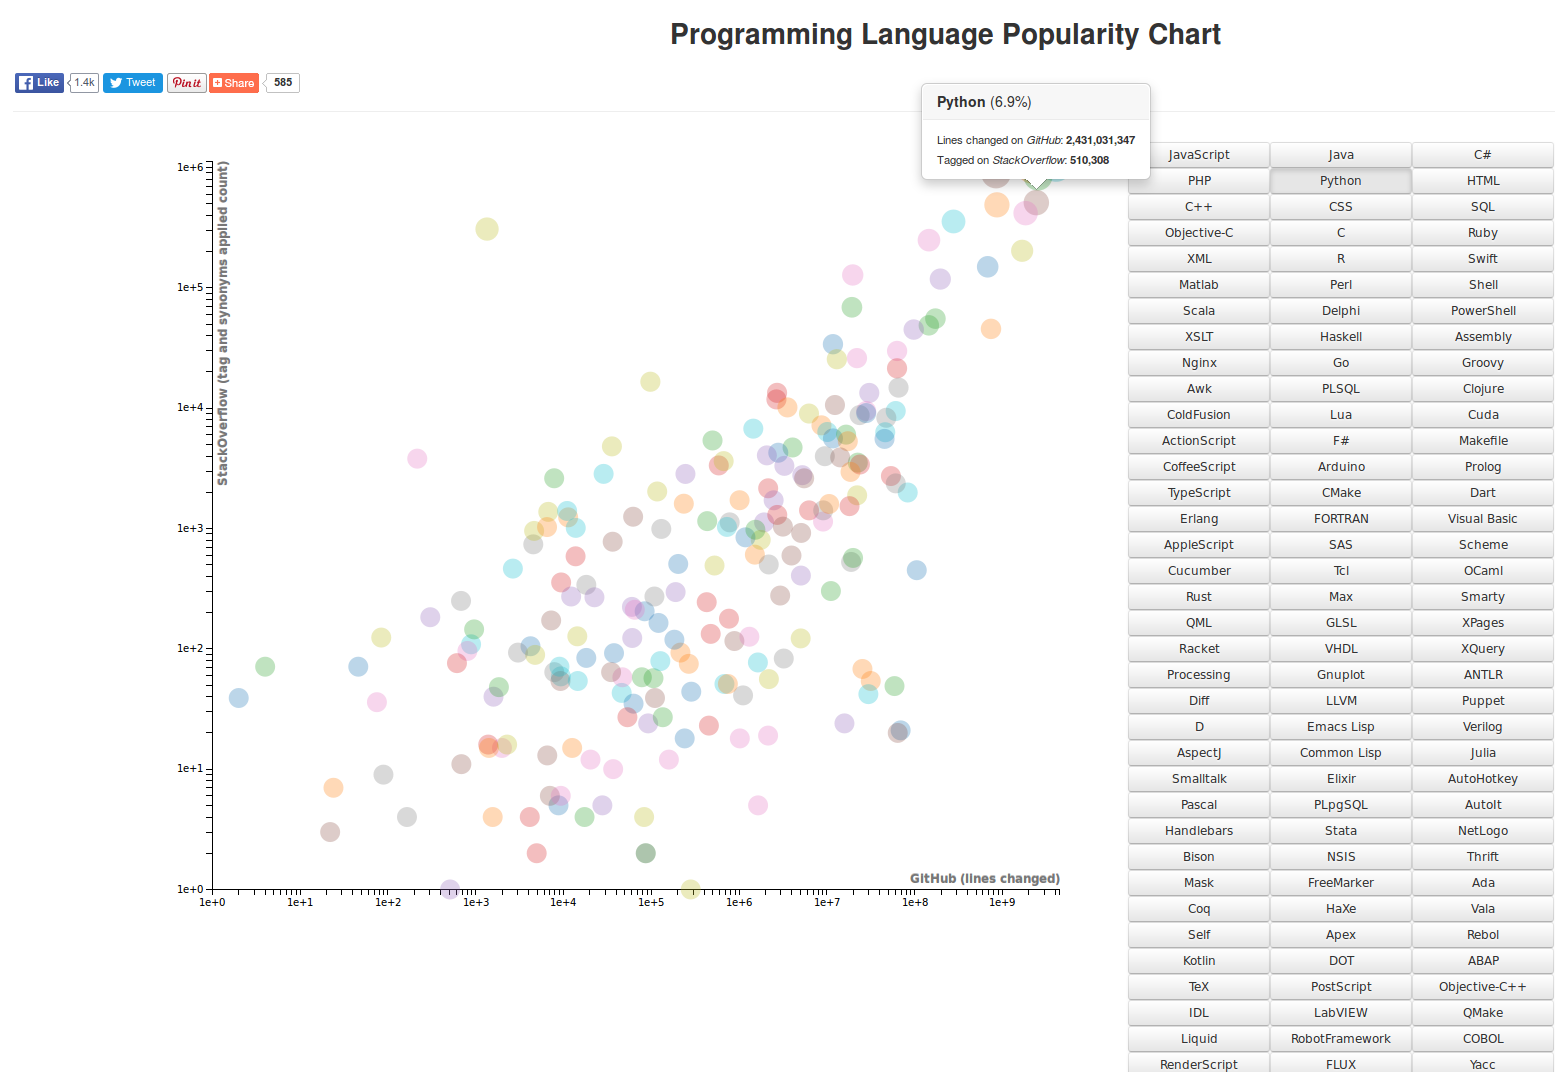
\includegraphics[width=.9\textwidth]{langpop_corger_nl}\\
{\scriptsize Source: \url{http://langpop.corger.nl/} (consulted in January 2016)}
}
\end{frame}



%--------------------------------------------------------------------------------------------------------------
\begin{frame}[c]
\frametitle{3 reasons not use Python?}


\begin{enumerate}
\item Don't have time to learn a new language
\item Slow? \comment{compared to C/C++, Fortran, Julia, \ldots}
\item Memory consumption
\end{enumerate}

\end{frame}


%--------------------------------------------------------------------------------------------------------------
\subsection{Python vs. MATLAB}

\begin{frame}[fragile]
\frametitle{Python vs. MATLAB}
\footnotesize

\begin{table}
\scriptsize
\begin{tabular}{p{.4\textwidth}p{.4\textwidth}}
\toprule
Python  	  				& MATLAB\\
\midrule
\textbf{General}			& \\
programming language		& programming language + numerical computing environment\\
open						& proprietary algorithms\\
general purpose				& linear algebra\\
\midrule
\textbf{Indexing} 			& 	\\
a[0]						& a(1) \\
a[-1]						& a(end)\\
a[::2]						& a(1:2:end)\\
\midrule
\textbf{Functions}			& \\
a.max()						& max(a)\\
a.shape()					& size(a)\\
\bottomrule
\end{tabular}
\end{table}

\vfill

Numpy for Matlab users:\\
\url{https://numpy.org/devdocs/user/numpy-for-matlab-users.html}

\end{frame}

%--------------------------------------------------------------------------------------------------------------
\begin{frame}[fragile]
\frametitle{Python 3 or Python 2}

\onslide*<1>{
\huge Python 3!!
}

\onslide*<2>{
Some differences:
\begin{itemize}
\item Print function
\item Integer division
\item Unicode
\item \ldots
\end{itemize}
}
\onslide*<3>{
\textit{"As of January 2020 Python 2 will be in EOL (End Of Life) status and receive no further official support."}

\vfill

More details:\\
\href{https://wiki.python.org/moin/Python2orPython3}{Python 2 or Python 3}\\
\href{https://jakevdp.github.io/blog/2013/01/03/will-scientists-ever-move-to-python-3/}{Will Scientists Ever Move to Python 3?}\comment{(January 2013)}
}

\end{frame}


%--------------------------------------------------------------------------------------------------------------
\begin{frame}[t, fragile]
\frametitle{Quick example: hello.py}

{\huge
\faLaptop
}


\begin{onlyenv}<2>
\begin{lstlisting}[language=python]
#!/usr/bin/python
"""
This function prints "Hello world"
"""

def hello():
  print("Hello world")
  return

def main():
  hello()

if __name__ == '__main__':
  main()
\end{lstlisting}
\end{onlyenv}

\end{frame}

\subsection{Running your code}

\begin{frame}[fragile, c]
\frametitle{Running your code: several solutions}

\begin{onlyenv}<1> 
Edit, then run in a shell:
\begin{lstlisting}[language=bash]
$ python mycode.py
\end{lstlisting}
or 
\begin{lstlisting}[language=bash]
$ mycode.py
\end{lstlisting}
if \textit{shebang} (\verb|#!|) is present at the 1st line
\begin{lstlisting}[language=python]
#!/usr/bin/python
\end{lstlisting}
\end{onlyenv}

\begin{onlyenv}<2> 
Interactive python (\href{http://ipython.org/}{ipython})

Auto-completion, exploring objects, \ldots

\begin{lstlisting}[language=bash]
In [2]: string = 'Hello all'

In [3]: string.
string.capitalize  string.encode      string.format      ...
string.rstrip      string.strip       string.upper       
... 
string.startswith  string.translate   
\end{lstlisting}

+ \textit{magic} functions:

{\footnotesize
\begin{itemize}
\item[] \verb|%run|: Run the named file inside IPython as a program\\
\item[] \verb|%timeit|: Time execution of a Python statement or expression\\
\item[] \verb|%who|: Print all interactive variables, with some minimal formatting
\end{itemize}
}
\vfill

More: \href{http://ipython.readthedocs.org/en/stable/interactive/magics.html?highlight=magic#built-in-magic-commands}{Built-in magic commands}
\end{onlyenv}

% Add ipython + magic functions + autocomplete etc

\begin{onlyenv}<3> 
\textit{Integrated Development Environment} (IDE)\\
(editor + build automation tools + debugger)

\vfill
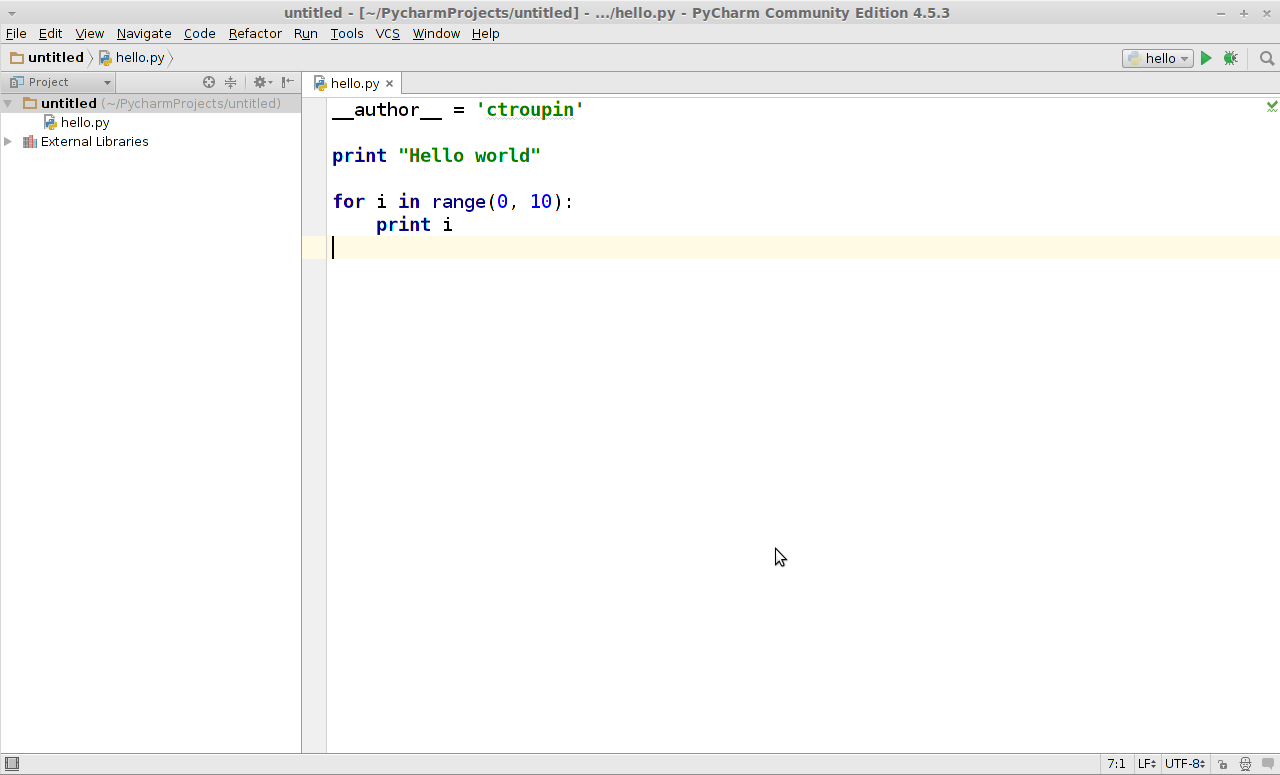
\includegraphics[width=.7\textwidth]{python_pycharm}
\vfill

\textbf{Examples:} Atom, Eclipse, PyCharm, Idle, \ldots\\
Complete list: \faLink~\url{https://wiki.python.org/moin/PythonEditors}
\end{onlyenv}

\begin{onlyenv}<4>
\href{https://jupyter.org/}{\textit{Jupyter notebook}}\\
(interactive computational environment)

\vfill
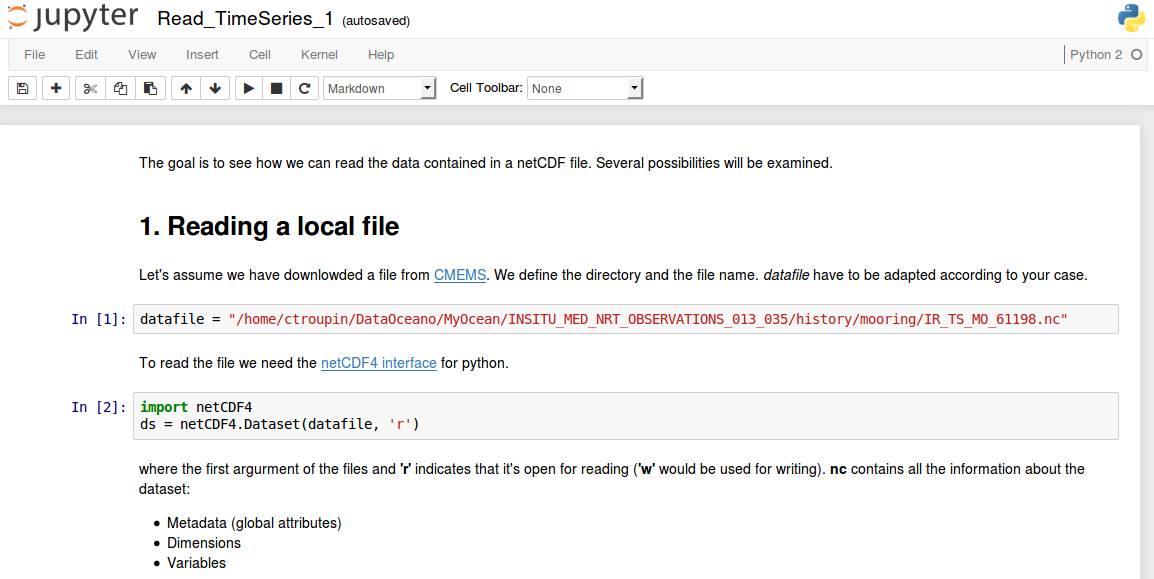
\includegraphics[width=.7\textwidth]{notebook_insitu0}
\vfill

Rich text + command executions + figures + \ldots

"\textit{Data story telling}"
\end{onlyenv}

\end{frame}

%--------------------------------------------------------------------------------------------------------------

\begin{frame}
\frametitle{Structure of a notebook}

\begin{columns}[c]

\begin{column}{.8\linewidth}
\begin{tikzpicture}
    \node[anchor=south west,inner sep=0] (image) at (0,0) {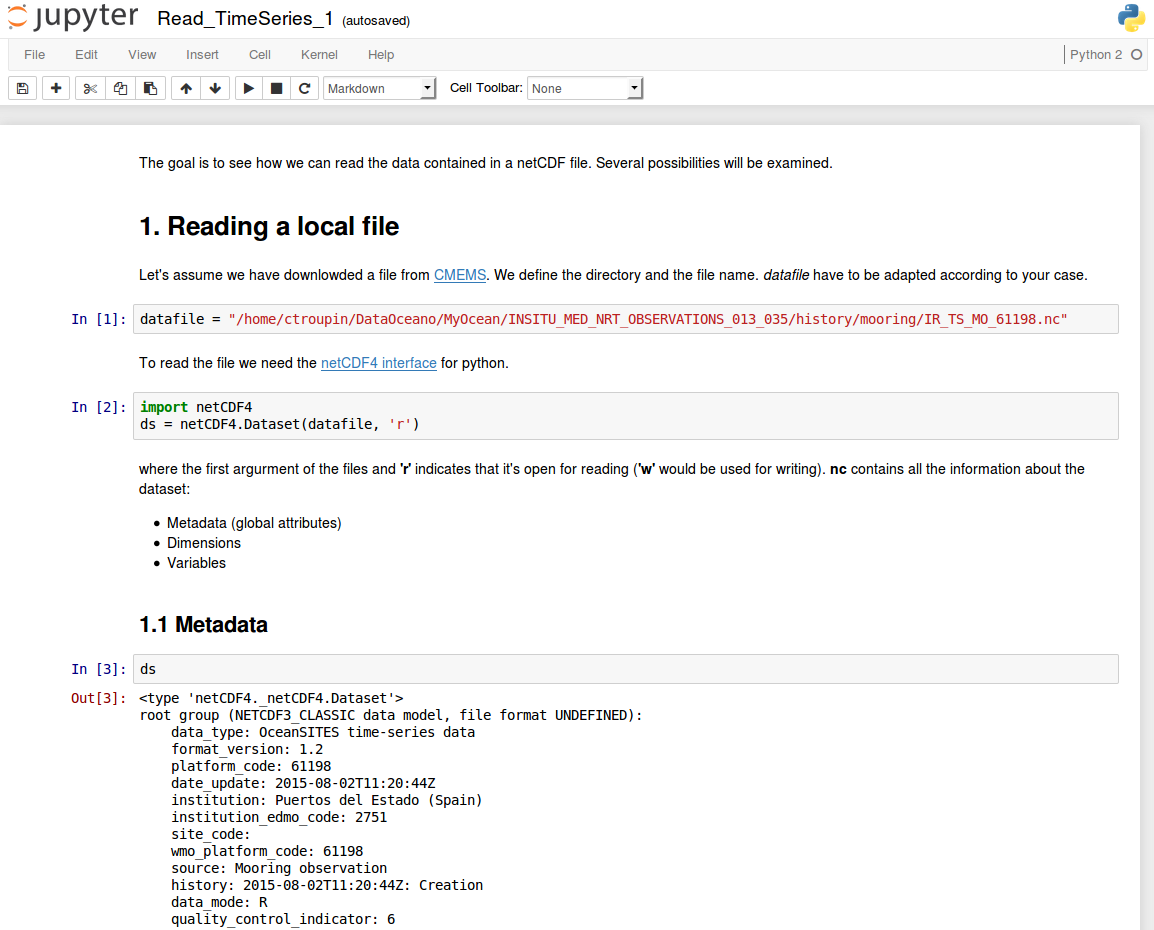
\includegraphics[width=.95\textwidth]{notebook_insitu1}};
    \begin{scope}[x={(image.south east)},y={(image.north west)}]
		\path (.21,.9) coordinate (play1);
		\path (.05,.9) coordinate (add1);
		\path (.35,.9) coordinate (cell1);
		\path (.05,.65) coordinate (code1);
		\path (.11,.49) coordinate (text1);
%		\draw[help lines,xstep=.1,ystep=.1] (0,0) grid (1,1);
%		\foreach \x in {0,1,...,9} { \node [anchor=north] at (\x/10,0) {0.\x}; }
%		\foreach \y in {0,1,...,9} { \node [anchor=east] at (0,\y/10) {0.\y}; }
    \end{scope}  
     
\end{tikzpicture}

\end{column}


\begin{column}{.25\linewidth}

\scriptsize 
\onslide<2->{\tikz[na] \coordinate (play2); Run current cell}

\onslide<3->{\tikz[na] \coordinate (add2); Add a new cell}

\onslide<4->{\tikz[na] \coordinate (cell2); Select type of cell}

\onslide<5->{\tikz[na] \coordinate (code2); Code cell}

\onslide<6>{\tikz[na] \coordinate (text2); Text cell}

\end{column}

\end{columns}

\begin{tikzpicture}[overlay]
\begin{scope}[x={(image.south east)},y={(image.north west)}]
	\onslide<2>{\path[*-stealth,arrowcolor,thin,opacity=0.25] (play1) edge [out=-90, in=180] (play2);}
	\onslide<3>{\path[*-stealth,arrowcolor,thin,opacity=0.25] (add1) edge [out=-90, in=180] (add2);}
	\onslide<4>{\path[*-stealth,arrowcolor,thin,opacity=0.25] (cell1) edge [out=-90, in=180] (cell2);}
	\onslide<5>{\path[*-stealth,arrowcolor,thin,opacity=0.25] (code1) edge [out=0, in=180] (code2);}
	\onslide<6>{\path[*-stealth,arrowcolor,thin,opacity=0.25] (text1) edge [out=0, in=180] (text2);}
\end{scope}
\end{tikzpicture}

\end{frame}


%--------------------------------------------------------------------------------------------------------------
\subsection{Definitions and data types}

%\begin{frame}[fragile]
%\frametitle{A few definitions}
%
%\begin{description}
%\item[Object:] Python's abstraction for data\\
%\url{https://docs.python.org/2/reference/datamodel.html#index-0}
%\item[Function:] series of statements which returns some value to a caller\\
%\url{https://docs.python.org/2/glossary.html#term-function}
%\item[Module:] file containing Python definitions and statements\\
%\url{https://docs.python.org/2/tutorial/modules.html}
%\item[Class:] logical grouping of data and methods (functions)\\
%\url{https://docs.python.org/2/tutorial/classes.html}
%\end{description}
%
%\end{frame}

%--------------------------------------------------------------------------------------------------------------

\begin{frame}[c]
\frametitle{Some data types}

Let's start to work!\\
\faLink~\href{../notebooks/Intro/data-types.ipynb}{Intro/data-types.ipynb}\\
\faLink~\href{../notebooks/Intro/control_flow.ipynb}{Intro/control\_flow.ipynb}

\end{frame}

%--------------------------------------------------------------------------------------------------------------
\subsection{Resources, tutorials, books}
\begin{frame}
\frametitle{Resources}

\onslide*<1>{
Web
\begin{itemize}
\item \url{https://docs.python.org/3/tutorial/}
\item \url{https://developers.google.com/edu/python/introduction?hl=en} \comment{tutorial + exercises}
\item \url{http://www.learnpython.org} \comment{online code execution}
\item \url{https://pythonprogramming.net}
\end{itemize}
}

\onslide*<2>{
Learning platforms
\begin{itemize}
\item \href{https://www.udacity.com/course/introduction-to-python--ud1110}{
Udacity: Introduction to Python Programming} \comment{(5 weeks)}
\item \href{https://www.codecademy.com/learn/python}{Code Academy} \comment{(25 hours)}
\item \href{https://www.datacamp.com/courses/intro-to-python-for-data-science}{DataCamp}
\end{itemize}
}

\onslide*<3>{
\faYoutube videos
\begin{itemize}
\item \href{https://www.youtube.com/watch?v=cpPG0bKHYKc}{Python Beginner Tutorial (For Absolute Beginners)}\comment{(4 parts)}
\item \href{https://www.youtube.com/watch?v=9uq3w6JJS00}{Zero to Hero with Python} \comment{(11 hours)}
\end{itemize}
}

\onslide*<4>{
\faBook books
\begin{itemize}
\item \textit{Learn Python the hard way}, Z.A.~Shaw, 2013\\
\url{http://learnpythonthehardway.org/book/}
\item \textit{Learning Python, 5th Edition}, M.~Lutz, 2013
\item \textit{Python Programming: An Introduction to Computer Science}, J.M. Zelle, 2002 
\end{itemize}

\vspace{1cm}

Complete list: \url{https://wiki.python.org/moin/PythonBooks}
}

\end{frame}


%--------------------------------------------------------------------------------------------------------------

\begin{frame}[fragile]
\frametitle{Objectives of the course}

\begin{enumerate}
\item<1-> Use Python to solve oceanography-related problems
\item<2-> Read/write various types of files
\item<3-> Generate high-quality figures
\end{enumerate}

\vspace{.5cm}

\onslide<5->{\textbf{What won't be done:}\\
make you a good programmer}

\end{frame}

%--------------------------------------------------------------------------------------------------------------

\begin{frame}
\frametitle{About the trainers}

\faLink~\href{../notebooks/Intro/teacher-map.ipynb}{Intro/teacher-map.ipynb}

\vspace{.2cm}

% maybe add pictures
\onslide<1->{\textbf{Arthur Capet}\\
Oceanographer\\
Post-doctoral researcher at \href{http://labos.ulg.ac.be/mast/}{MAST}\\
4-year experience with Python

}

\vspace{1cm}

\onslide<2->{\textbf{Charles Troupin}\\
Engineer, oceanographer\\
Post-doctoral researcher at \href{http://labos.ulg.ac.be/gher/}{GHER}\\
7-year experience with Python
}

\end{frame}

%--------------------------------------------------------------------------------------------------------------

\begin{frame}[t]
\frametitle{Content of the course}

\begin{enumerate}
\item<1-> Reading/writing data files
\item<2-> Working with time series 
\item<3-> Plotting 2-D fields
\item<4-> Functions, classes, modules
\end{enumerate}

\vspace{1cm}

\includegraphics<1->[height=2cm]{python_idle2}~\includegraphics<2->[height=2cm]{IR_TS_MO_61198_monthly}\\
\includegraphics<3->[height=2cm]{anomalies_10profiler-glider_201507}~\includegraphics<4->[height=2cm]{eddy_tracking_ex}

\end{frame}

